% The contact list in your phone is sorted, which means you can easily access your desired contact from your phone since the data is arranged in that manner for you. In other words, “it is sorted”.

% While shopping on flip kart or amazon, you sort items based on your choice, that is, price low to high or high to low.

% used in programming TV to sort channels based on audience viewing time!
% \section{Nomenclatura}
% Una llista és una seqüència de qualsevol valor. Per exemple: $llistaA: 4, 5, 6, 7$. La \textit{llistaA} és una llista ordenada ascendentment de nombres naturals consecutius amb 4 elements.

% Per accedir a cada element de la llista utilitzarem la seva posició o índex començant per 0. Ho podem expressar d'aquesta manera per exemple, $llistaA[0] = 4$. A l'índex 0 de la \textit{llistaA} hi ha l'element 4.
% \begin{figure}[h]
%     \begin{center}
%     \renewcommand{\arraystretch}{1.5}
%     \begin{tabular}{|c | c | c | c | c |} 
%      \hline
%      \textit{LlistaA} & 4 & 5 & 6 & 7 \\ 
%      \hline
%      Índex & 0 & 1 & 2 & 3 \\
%      \hline
%     \end{tabular}
%     \end{center}
%     \caption{Llistes i posicions.}
%     \label{fig:my_label}
% \end{figure}    

% En aquesta llista hi ha $n = 4$ elements, així que el primer element és $LlistaA[0]$, i l'últim element és $LlistaA[n-1]$.

% Per tant, per obtenir tots els elements de la llista, haurem de mirar tots els índexs entre 0 i $n-1$ ambdós inclosos.

Hi ha dos problemes bàsics i essencials que han de poder resoldre tots els dispositius. Aquests són: la cerca i l'ordenació. L'ordenació consisteix a ordenar un conjunt de dades. I la cerca consisteix a trobar la posició d'una dada en un conjunt.

Com tots els problemes hi ha moltes formes de solucionar-los, per això explicaré dos algoritmes per cada problema i els analitzarem per determinar el més eficient. En el següent capítol implementarem els algoritmes.

% Aquests dos problemes els trobem en moltes situacions, per exemple: les paraules d'un diccionari estan ordenades per facilitar la cerca d'una paraula. Quan ordenem el menjar segons la data de caducitat. O quan ordenem els valors de la borsa en funció dels beneficis en un període de temps determinat. O quan busques una paraula en un document, quan cerques un producte a la pàgina d'una botiga... 

Aquests dos problemes els podem trobar en algoritmes que resolen tasques més complexes i que en el seu funcionament requereixen resoldre aquestes tasques més simples. I per optimitzar aquests algoritmes més complexos, podem començar optimitzant una part de l'algoritme com pot ser la resolució d'una cerca o ordenació.
\section{Cerca}
Aquest problema consisteix a trobar la posició d'una dada en un conjunt. En aquest treball, per simplicitat, utilitzarem un conjunt d'$n$ nombres enters. Per tant, aquest problema té dues entrades: el nombre que cerquem, que anomenarem $k$, i una llista o seqüència d'$n$ nombres. 

Com que la sortida del problema és la posició o índex de $k$ a la llista, hem de definir quin índex té cada nombre. En programació normalment es comença a indexar des de zero, així que el primer element té índex 0, el segon té índex 1 així fins a $n-1$. Per exemple:
\begin{figure}[h]
    \begin{center}
    \renewcommand{\arraystretch}{1.5}
    \begin{tabular}{|c | c | c | c | c |} 
     \hline
     \textit{Llista} & 48 & 5 & 12 & 83 \\ 
     \hline
     Índex & 0 & 1 & 2 & 3 \\
     \hline
    \end{tabular}
    \end{center}
    \caption{Llistes i índex.}
    \label{fig:my_label}
\end{figure} 

Veiem com la llista té $n = 4$ elements, així que l'últim element té l'índex d'$n-1 = 4-1 = 3$. 

Per exemple, si les entrades d'un problema de cerca són la llista de la figura 2.1, i $k = 5$. Hem de trobar la posició de $k = 5$ en la $Llista = \lbrace 48, 5, 12, 83 \rbrace$. De manera que la sortida seria 1. Ja que la posició de $k = 5$ en la llista té índex = 1. També ho podriem expressar com $Llista_1 = 5$, ja que a l'índex 1 de la llista hi ha l'element 5.

\subsection{Cerca lineal}
L'algoritme de cerca lineal consisteix a mirar cada element un per un i comprovar si coincideixen amb el que estem buscant ($k$). Aquest algoritme acaba quan trobem l'element o hem comprovat tota la llista.

% Com diu el nom de l'algoritme, té complexitat lineal. De fet, l'exemple de complexitat lineal del capítol anterior és un algoritme de cerca lineal. 
Per exemple, si tenim una $Llista = \lbrace 6, 2, 1, 8, 4 \rbrace$ i $k = 8$. L'algoritme faria el següent:

Anomenem $i$ l'índex del nombre que estem comprovant ($i$ incrementa a cada pas). Així, quan es compleix $Llista_i = k$, la sortida serà igual a $i$.

\begin{enumerate}
    \item Comprova el primer element ($Llista_0 = 6$), com que aquest no és igual a $k = 8$, passa al següent, $i = i + 1$.
    \item $Llista_1 = 2$, com que $2 \neq k$, passa al següent.
    \item Després comprova $i = 2$ com que $Llista_2 \neq k$ comprovem el següent.
    \item Finalment $Llista_3 = k$, la sortida és $i = 3$ i acaba l'algoritme.
\end{enumerate}

Ho podem representar gràficament amb la figura 2.2.
% \begin{wrapfigure}[7]{R}{.45\textwidth}
\begin{figure}[h]
    % \vspace{-18pt}
    \centering
    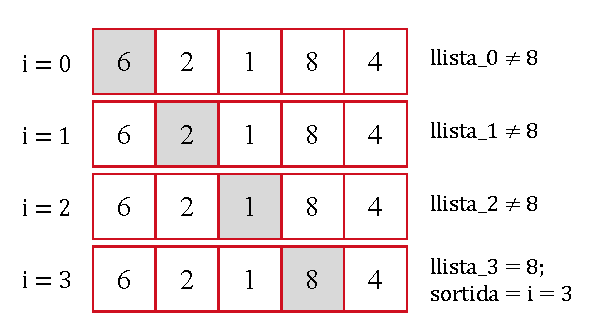
\includegraphics[width=.45\textwidth]{capitols/figures/linearsearch (2).pdf}
    \caption[Cerca lineal.]{Cerca lineal. Font: elaboració pròpia.}
    \label{fig:my_label}
\end{figure}

Pot passar que l'element no estigui a la llista, en aquest cas comprovaríem els $n$ elements i quan acabés la llista, acabaria l'algoritme.

El pitjor cas possible de la cerca lineal és que l'element se situï en l'última posició o que no hi sigui a la llista. En ambdós casos hauríem de comprovar els $n$ elements, per això aquest algoritme té complexitat lineal o $O(n)$. Les operacions per comparar si l'element coincideix, són constants (no depenen d'$n$), per això les podem eliminar de l'analisi de complexitats.

La implementació de la cerca lineal la podeu trobar a \textcolor{red}{l'annex 2.}

\subsection{Cerca dicotòmica}
L'algoritme de la cerca dicotòmica resol el mateix problema que la cerca lineal, però amb el requisit que la llista ha d'estar ordenada. Aquest algoritme és el mateix que el de l'exemple del diccionari de la complexitat logarítmica. 

Aquest algoritme consisteix a acotar el rang on podem trobar l'element fins que només en queda un i coincideix amb el que busquem. Per acotar el rang partim la llista per la meitat, i com que està ordenada, podem saber en quina meitat es troba $k$, de manera que a cada pas podem descartar la meitat dels elements que ens quedaven.

% \begin{wrapfigure}[7]{R}{.52\textwidth}
%     \vspace{-18pt}
%     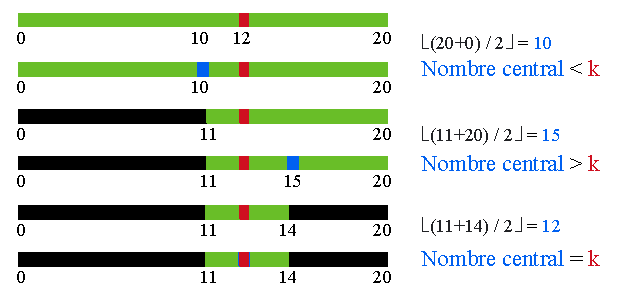
\includegraphics[width=.52\textwidth]{capitols/figures/binarysearch (2).pdf}
%     \caption[Exemple 1. Cerca dicotòmica.]{Exemple 1. Cerca dicotòmica. Font: elaboració pròpia.}
%     \label{fig:my_label}
% \end{wrapfigure}

% En la figura 2.3 hi ha un exemple en que $n = 21$ i $k = 12$. Inicialment, $k$ (franja vermella) pot estar en el rang sencer de la llista (franja verda), ja que encara no hem fet cap operació. El primer que fa l'algoritme és trobar el nombre central (franja blava) del rang 0 - 20 que és 10, i com que $k > 10$ podem suposar que $k$ està a la dreta del nombre central. Així que podem acotar el rang, $k$ es troba entre el nombre central exclòs i el nombre més gran, és a dir, 11 - 20. Ara repetim el mateix, però amb el nombre central d'entre 11 i 20 que és 15. Com que $k < 15$ sabem que $k$ està a l'esquerra del nombre central, entre 11 i 14, ja que excloem el 15. Repetim el mateix en el rang 11 - 14, el centre és 12. Com que $k = 12$, ja hem trobat el nombre i acaba l'algoritme.

% Tot aquest procés es realitza amb els índexs dels nombres de la llista, d'aquesta manera, no cal que els nombres siguin consecutius, només cal que estiguin ordenats. 

% En l'exemple de la figura 2.3, per simplicitat i perquè s'entengui millor l'algoritme, els nombres són consecutius de 0 a 20, de manera que els índexs coincideixen amb els valors. Normalment, la llista no és de nombres consecutius de manera que no pots suposar la posició del valor que busques. L'exemple de la figura 2.4 és més acurat.

Per exemple, si tenim la $Llista = \lbrace 2, 4, 7, 12, 24, 38, 51, 56, 62, 65, 71, 83, 89, 98, 99 \rbrace$, $n = 15$ i $k = 62$. L'algoritme faria el següent:

% En la figura 2.4 $k$ pot estar en el rang sencer, 0 - 14, i la dada del centre és a l'índex $\frac{0+14}{2} = 7$. $Llista_7 = 56$, $56 < k$, així que sabem que $k$ estarà entre l'índex 8 i el 14. La dada central d'aquest rang és $\frac{8+14}{2} = 11$, $Llista_{11} = 83$, $83 > k$. Per tant, sabem que $k$ està en un índex més petit o igual a 10 i més gran o igual a 8. Així que el centre és $\frac{8+10}{2} = 9$, $Llista_9 = 65, 65 > k$ així que sabem que $k$ està entre 8 i 8. Com que $Llista_8 = 62 = k$, acabem l'algoritme i la sortida és 8.

\begin{enumerate}
\item $k$ es troba en el rang 0 - 14 ambdós inclosos, per tant,  calculem en quin índex queda la dada central, així, $\frac{0+14}{2} = 7$. Com que $k$ és més gran que la dada de l'índex 7, podem descartar totes les posicions més petites a l'índex 7 inclòs. És a dir, com que $Llista_7 = 56 < k$  podem assegurar que $k$ es troba en el rang 8 - 14 ambdós inclosos.
\item Repetim el pas 1 però en el rang 8 - 14 ambdós inclosos. La dada central es troba a l'índex $\frac{8+14}{2} = 11$. Com que $LLista_{11} = 83 > k$, $k$ es troba a l'esquerra de l'índex 11, en el rang 8 - 10 ambdós inclosos. 
\item Trobem la dada central de 8 - 10, $\frac{8+10}{2} = 9$, $Llista_9 = 65 > k$ . Per tant, $k$ es troba en el rang 8 - 8.
\item La dada central de 8 - 8 es troba en $\frac{8+8}{2} = 8$, $Llista_8 = 62 = k$. Per tant, acaba l'algoritme i la sortida és 8. 
\end{enumerate}

Ho podríem representar gràficament en la figura 2.3. Els elements en verd representen els que no han estat descartats, els que estan en blau representen les dades centrals, i en vermell representen $k$.

\begin{figure}[h]
    \centering
    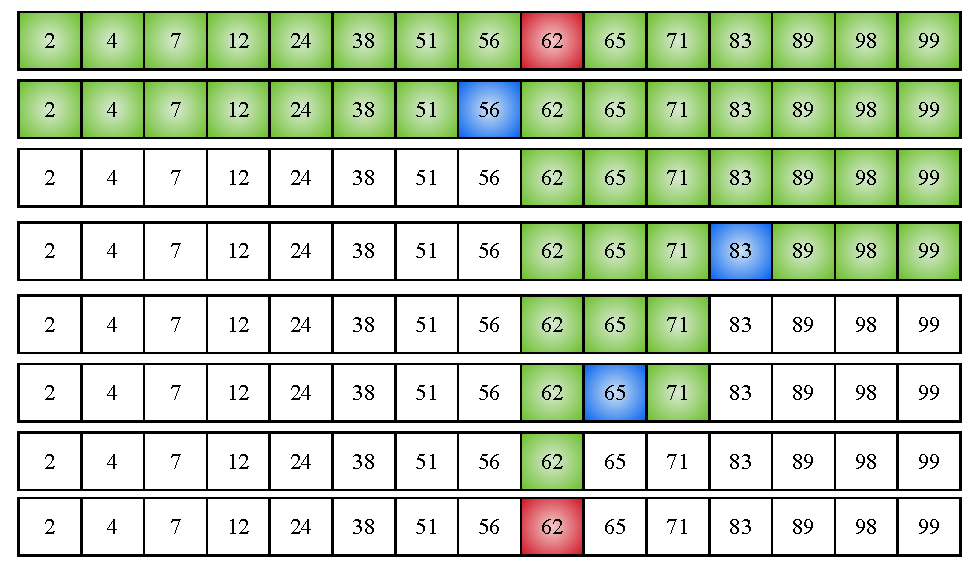
\includegraphics[width=.65\textwidth]{capitols/figures/binary2.pdf}
    \caption[Exemple 2. Cerca dicotòmica.]{Exemple 2. Cerca dicotòmica. Font: elaboració pròpia.}
    \label{fig:my_label}
\end{figure}
El pitjor cas possible és que $k$ no es trobi a la llista, ja que hauríem d'arribar a partir les dades d'una en una per assegurar-nos que no ho estigui. Això també ha passat en l'exemple de la figura 2.3, encara que $k$ estigués a la llista. En canvi, si haguéssim escollit $k = 82$, haguésim acabat l'algoritme partint les dades una sola vegada.

Com hem explicat al punt 1.2.2 a la complexitat logarítmica, aquest algoritme té complexitat logarítmica, ja que $\lceil\log_2{n}\rceil$ és la quantitat necessària de passos per partir les dades de la manera com ho fa la cerca dicotòmica. En la figura 1.7 es pot veure com es parteixen les dades igual que en aquest algoritme, i la relació que té amb els logaritmes.

Com hem vist, a cada partició de les dades s'ha de buscar la dada central i resoldre una inequació. Com que aquestes operacions són constants (no depenen d'$n$), les podem eliminar de l'analisi de complexitats, i ens queda que aquest algoritme té complexitat $O(\log_2{n})$.

La implementació de la cerca dicotòmica la podeu trobar a \textcolor{red}{l'annex 3.}

\section{Ordenació}
Els problemes d'ordenació consisteixen a ordenar un conjunt de dades. En aquest treball ordenarem ascendentment nombres enters.

L'entrada d'aquest problema és una llista d'$n$ elements. I la sortida consisteix en els $n$ elements ordenats ascendentment.

Hi ha molts algoritmes diferents per resoldre aquest problema, i tots tenen avantatges i inconvenients. En aquest treball ens centrem només en l'eficiència temporal, però hi ha molts altres factors que també afecten l'eficiència de l'algoritme i depèn de la situació cal tenir-ho en conte. N'hi ha que són molt ràpids, però ocupen molta memòria (ordenació per barreja), en canvi, n'hi ha que són més lents, però ocupen menys memòria (ordenació de bombolla), n'hi ha que són més ràpids si hi ha moltes dades repetides, n'hi ha que són específics per a estructures de dades determinades (llistes, heaps, grafs, maps...).

\subsection{Ordenació de bombolla}
Aquest algoritme consisteix a intercanviar dos elements adjacents si no estan en ordre.

Per exemple, si tenim una $Llista = \lbrace7, 2, 5, 3, 11\rbrace$ i $n = 5$, l'algoritme faria el següent:

\begin{enumerate}
    \item Comprovem el primer i segon element (7 i 2), com que $7 > 2$ els intercanviem. I ens queda $Llista = \lbrace2, 7, 5, 3, 11\rbrace$.
    \item Comprovem el segon i tercer element. Com que $7 > 5$, els intercanviem. I queda $Llista = \lbrace2, 5, 7, 3, 11\rbrace$.
    \item Comprovem el tercer i quart element. Com que $7 > 3$, els intercanviem. I queda $Llista = \lbrace2, 5, 3, 7, 11\rbrace$.
    \item Comprovem el quart i cinquè element. Com que $7 < 11$, no els intercanviem. I la llista queda igual $Llista = \lbrace2, 5, 3, 7, 11\rbrace$.
    \item Ara ja hem acabat la llista, i hem de repetir el mateix procediment $n$ vegades en total. \\ Comprovem el primer i segon element. Com que $2 < 5$, queden igual. I queda $Llista = \lbrace2, 5, 3, 7, 11\rbrace$.
    \item Comprovem el segon i tercer element. Com que $5 > 3$, els intercanviem. I queda $Llista = \lbrace2, 3, 5, 7, 11\rbrace$.
    \item Ara la llista ja està ordenada, però els ordinadors no ho poden saber si no ho comproven. I no ho comproven perquè això faria l'algoritme molt lent, ja que cada comprovació té complexitat lineal. Això fa que en un ordinador aquest algoritme segueixi funcionant fins a repetir aquest procés un total d'$n$ vegades, encara que no es canviarà d'ordre cap dada. De manera que no hi ha un pitjor cas possible, ja que en tots els casos es farà la mateixa quantitat d'operacions.
\end{enumerate}

Aquest algoritme itera tota la llista d'$n$ elements $n$ vegades, per tant, fa $n \cdot n = n^2$ operacions. Per això aquest algoritme té complexitat quadràtica o $O(n^2)$. 

Igual que en la cerca, l'algoritme resol inequacions que tenen complexitat constant, i, per tant, no cal tenir-les en compte, ja que depenen de l'ordinador.

\subsection{Ordenació per barreja} %merge
El funcionament d'aquest algoritme el podríem partir en dues parts: en la primera part parteix les dades igual que en la cerca dicotòmica (figura 2.4), i en la segona part les ajunta fins que queden en una sola llista ordenades (figura 2.5). Així:

\begin{figure}[H]
    \centering
    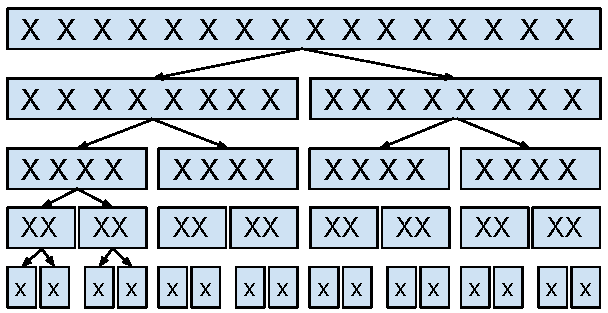
\includegraphics[width=.6\textwidth]{capitols/figures/merge.pdf}
    \caption[Divisió de les dades.]{Divisió de les dades. Font: elaboració pròpia.}
    \label{fig:my_label}
\end{figure}
\vspace{-.8cm}
En la figura 2.4 podem veure com cada llista es parteix per la meitat fins a quedar dades individuals. Igual que en la cerca dicotòmica, i, per tant, també té complexitat logarítmica.
% \vspace{-.5cm}
\begin{figure}[H]
    \centering
    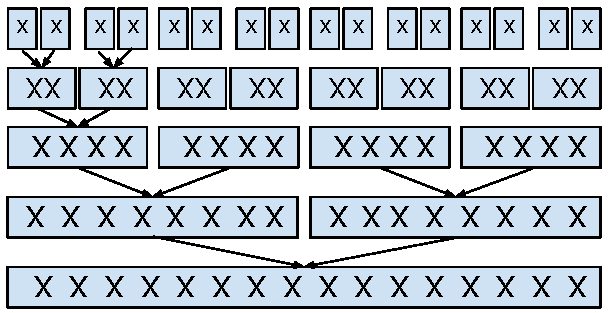
\includegraphics[width=.6\textwidth]{capitols/figures/merge2.pdf}
    \caption[Ajuntar les dades.]{Ajuntar les dades. Font: elaboració pròpia.}
    \label{fig:my_label}
\end{figure}
\vspace{-.5cm}
\begin{wrapfigure}[10]{R}{.35\textwidth}
\vspace{-18pt}
    \centering
    \includegraphics[width=.35\textwidth]{capitols/figures/Còpia de merge2.pdf}
    \caption[Exemple d'ajuntar les dades.]{Exemple d'ajuntar les dades. Font: elaboració pròpia.}
    \label{fig:my_label}
\end{wrapfigure}
Ajuntar les dades és molt simple. Com que comencem amb dades individuals sempre són grups de dades ordenades, per això les podem ordenar tan ràpidament. Primer mirem la dada més petita dels dos grups que volem ajuntar, és a dir, la primera. Després posem la més petita de les dues a la següent llista i avancem una posició a la llista d'on hem tret la dada. Ho podem representar gràficament amb la figura 2.6.

Aquest procediment es repeteix cada vegada que s'ajunten dues llistes.

Podem posar un exemple d'aquest algoritme per a $n = 8$ i $Llista = \lbrace5, 2, 4, 7, 1, 3, 2, 6\rbrace$ en la figura 2.7.

\begin{figure}[H]
    \centering
    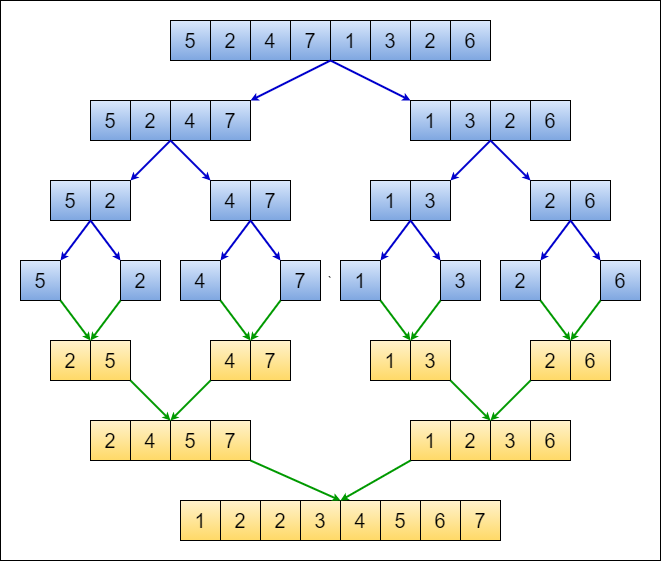
\includegraphics[width=.5\textwidth]{capitols/figures/merge5.png}
    \caption[Exemple d'ordenació per barreja.]{Exemple d'ordenació per barreja. Font: https://levelup.gitconnected.com/visualizing-designing-and-analyzing-the-merge-sort-algorithm-cf17e3f0371f.}
    \label{fig:my_label}
\end{figure}

\vspace{-18pt}
En la primera part de l'algoritme (part blava) només es parteixen les dades, i en la segona part (part groga) s'ajunten com hem vist a la figura 2.6 fins a obtenir una sola llista.

Analitzarem la complexitat d'aquest algoritme separant la part blava de la groga, i després sumarem els dos resultats. La part blava com ja hem vist anteriorment té complexitat logarítmica. I la part groga té complexitat $O(n \cdot log_2{n})$.

En la figura 2.6 hem ajuntat dues llistes de 3 elements per obtenir una llista d'$n = 6$, i hem fet $n$ operacions, ja que hem recorregut cada llista una vegada. De manera que el procediment d'ajuntar dues llistes té complexitat lineal.

En la part groga de la figura 2.7 hi ha les mateixes particions que en la part blava però invertides. És a dir, hi ha $\log_2{n}$ passos a la part groga, i a cada pas ajuntem els $n$ elements de forma lineal. Els ajuntem en llistes diferents de mides diferents, però la suma d'aquestes subllistes tenen mida $n$. Així que en total fem un procediment lineal $\log_2{n}$ vegades, o expressat d'una altra manera $O(n \cdot \log_2{n})$.

Si ho ajuntem tot ens queda una complexitat de $O(\log_2{n} + n \cdot \log_2{n}) \equiv O(n \cdot \log_2{n})$, ja que en l'últim pas podem eliminar el primer $\log_2{n}$ ja que és un terme de creixement més lent.

